\documentclass{beamer}

\usetheme{dtyped}

\usepackage{hyperref}
\hypersetup{
  colorlinks=true,
  allcolors=.,
  urlcolor=blue,
}
\usepackage[
  backend=biber,
  style=numeric,
  isbn=false,
  url=false,
  doi=false
]{biblatex}
\addbibresource{citations.bib}
\usepackage{listings}
\lstset{ 
  backgroundcolor=\color{white},   % choose the background color; you must add \usepackage{color} or \usepackage{xcolor}; should come as last argument
  basicstyle=\footnotesize\ttfamily,
  breakatwhitespace=false,         % sets if automatic breaks should only happen at whitespace
  breaklines=true,                 % sets automatic line breaking
  captionpos=b,                    % sets the caption-position to bottom
  commentstyle=\itshape\color{gray},     % comment style
  extendedchars=true,              % lets you use non-ASCII characters; for 8-bits encodings only, does not work with UTF-8
  keepspaces=true,                 % keeps spaces in text, useful for keeping indentation of code (possibly needs columns=flexible)
  keywordstyle=\bfseries\color{black},      % keyword style
  numbers=left,                    % where to put the line-numbers; possible values are (none, left, right)
  numbersep=5pt,                   % how far the line-numbers are from the code
  numberstyle=\tiny\color{gray}, % the style that is used for the line-numbers
  showspaces=false,                % show spaces everywhere adding particular underscores; it overrides 'showstringspaces'
  showstringspaces=false,          % underline spaces within strings only
  showtabs=false,                  % show tabs within strings adding particular underscores
  stringstyle=\color{gray},      % string literal style
  tabsize=2,	                   % sets default tabsize to 2 spaces
  title=\lstname,                  % show the filename of files included with \lstinputlisting; also try caption instead of title
  belowskip=-0.8 \baselineskip
}

% from https://tex.stackexchange.com/questions/178800/creating-sections-each-with-title-pages-in-beamers-slides
\AtBeginSection[]{
  \begin{frame}
  \vfill
  \centering
\begin{beamercolorbox}[sep=8pt,center,shadow=true,rounded=true]{title}
    \usebeamerfont{title}\insertsectionhead\par%
  \end{beamercolorbox}
  \vfill
  \end{frame}
}

% https://tex.stackexchange.com/questions/220707/using-scalebox-to-decrease-the-size-of-listings-code
\newsavebox{\mybox}

\title{\texttt{dependently-typed}}
\subtitle{A programming languages club at Georgia Tech}
\author{Elton Pinto}
\date{\today}

\begin{document}

\begin{frame}
  \titlepage
\end{frame}

\begin{frame}
  \begin{center}
    Slides available at \\
    \small\url{https://github.com/dependently-typed/promo}
  \end{center}
\end{frame}

\begin{frame}[fragile]{Question for you}
  Have you ever wondered how your code magically runs?

  \vspace{1cm}

  \begin{lstlisting}[language=Python]
def fibonacci(n):
    if n <= 0:
        return 1
    else:
        return fibonacci(n-1) + fibonacci(n-2)
  \end{lstlisting}
\end{frame}

\begin{frame}[fragile]{}
  Surprise, surprise. It's not magic :)
  \vspace{1cm}

  \begin{lrbox}{\mybox}%
    \begin{lstlisting}[language=Python]
  2           0 LOAD_FAST                0 (n)
              2 LOAD_CONST               1 (0)
              4 COMPARE_OP               1 (<=)
              6 POP_JUMP_IF_FALSE        6 (to 12)

  3           8 LOAD_CONST               2 (1)
             10 RETURN_VALUE

  5     >>   12 LOAD_GLOBAL              0 (fibonacci)
             14 LOAD_FAST                0 (n)
             16 LOAD_CONST               2 (1)
             18 BINARY_SUBTRACT
             20 CALL_FUNCTION            1
             22 LOAD_GLOBAL              0 (fibonacci)
             24 LOAD_FAST                0 (n)
             26 LOAD_CONST               3 (2)
             28 BINARY_SUBTRACT
             30 CALL_FUNCTION            1
             32 BINARY_ADD
             34 RETURN_VALUE
    \end{lstlisting}
  \end{lrbox}%
  
  \begin{columns}[b]
    \begin{column}{0.4\textwidth}
      \begin{figure}
      \scalebox{0.5}{\usebox{\mybox}}
      \caption{Python bytecode for \texttt{fibonacci}}
      \end{figure}
    \end{column}
    \begin{column}{0.4\textwidth}
      \begin{figure}
        \raisebox{0.25\height}{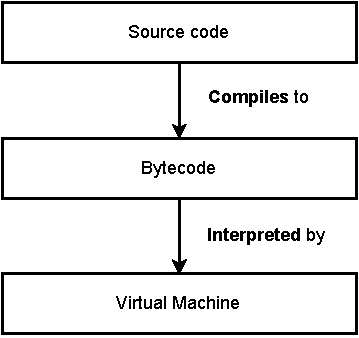
\includegraphics[width=0.8\textwidth]{assets/python-interpreter-overview}}
      \caption{Python runtime overview}
      \end{figure}
    \end{column}
  \end{columns}
\end{frame}

\begin{frame}{About the club}
  \begin{columns}
    \begin{column}{0.8\textwidth}
      \begin{itemize}
      \item Programming languages (PL) and compilers club
      \item Open to undergraduate and graduate students
      \item Weekly meetings on Tuesday, 6-7pm CCB 340
      \end{itemize}
    \end{column}

    \begin{column}{0.15\textwidth}
      \centering
      
\includegraphics[width=\textwidth]{assets/dragon.png}
    \end{column}
  \end{columns}
\end{frame}

\begin{frame}{What do we do?}
  \begin{itemize}
  \item Talks, workshops, and paper reading sessions
  \item Networking and community building
  \item Projects
  \end{itemize}
\end{frame}

\begin{frame}{Talks}
  \begin{itemize}
    \item Student driven, with occasional guest speakers
    \item Member talks:
      \begin{itemize}
        \item What the f*** is a monad?
        \item Fast in-place interpreter for WebAssembly
        \item Types and propositions / intro to constructive logic
      \end{itemize}
    \item Guest talks:
      \begin{itemize}
        \item Vivek Sarkar (chair of SCS) gave a talk about his research on parallelizing Python for large-scale data processing
        \item Nathan Braswell gave a talk about his work on F-expression compilation
        \item Sharjeel Khan gave a talk about his journey into PL research
      \end{itemize}
    \item Schedule: \url{https://dtyped.netlify.app/wiki/schedule}
  \end{itemize}
\end{frame}

\begin{frame}{Why should I care?}
  \begin{itemize}
    \item Programming languages and compilers are everywhere, and are here to stay.
    \item You will stand out. `Tis a very marketable set of skills to employers.
    \item The knowledge you will gain is broadly applicable to and is heavily
      used in other fields of CS.
  \end{itemize}
\end{frame}

\begin{frame}{If not for anything else...}
  You'll learn how to give \textit{life} to the inanimate.
  \begin{figure}
  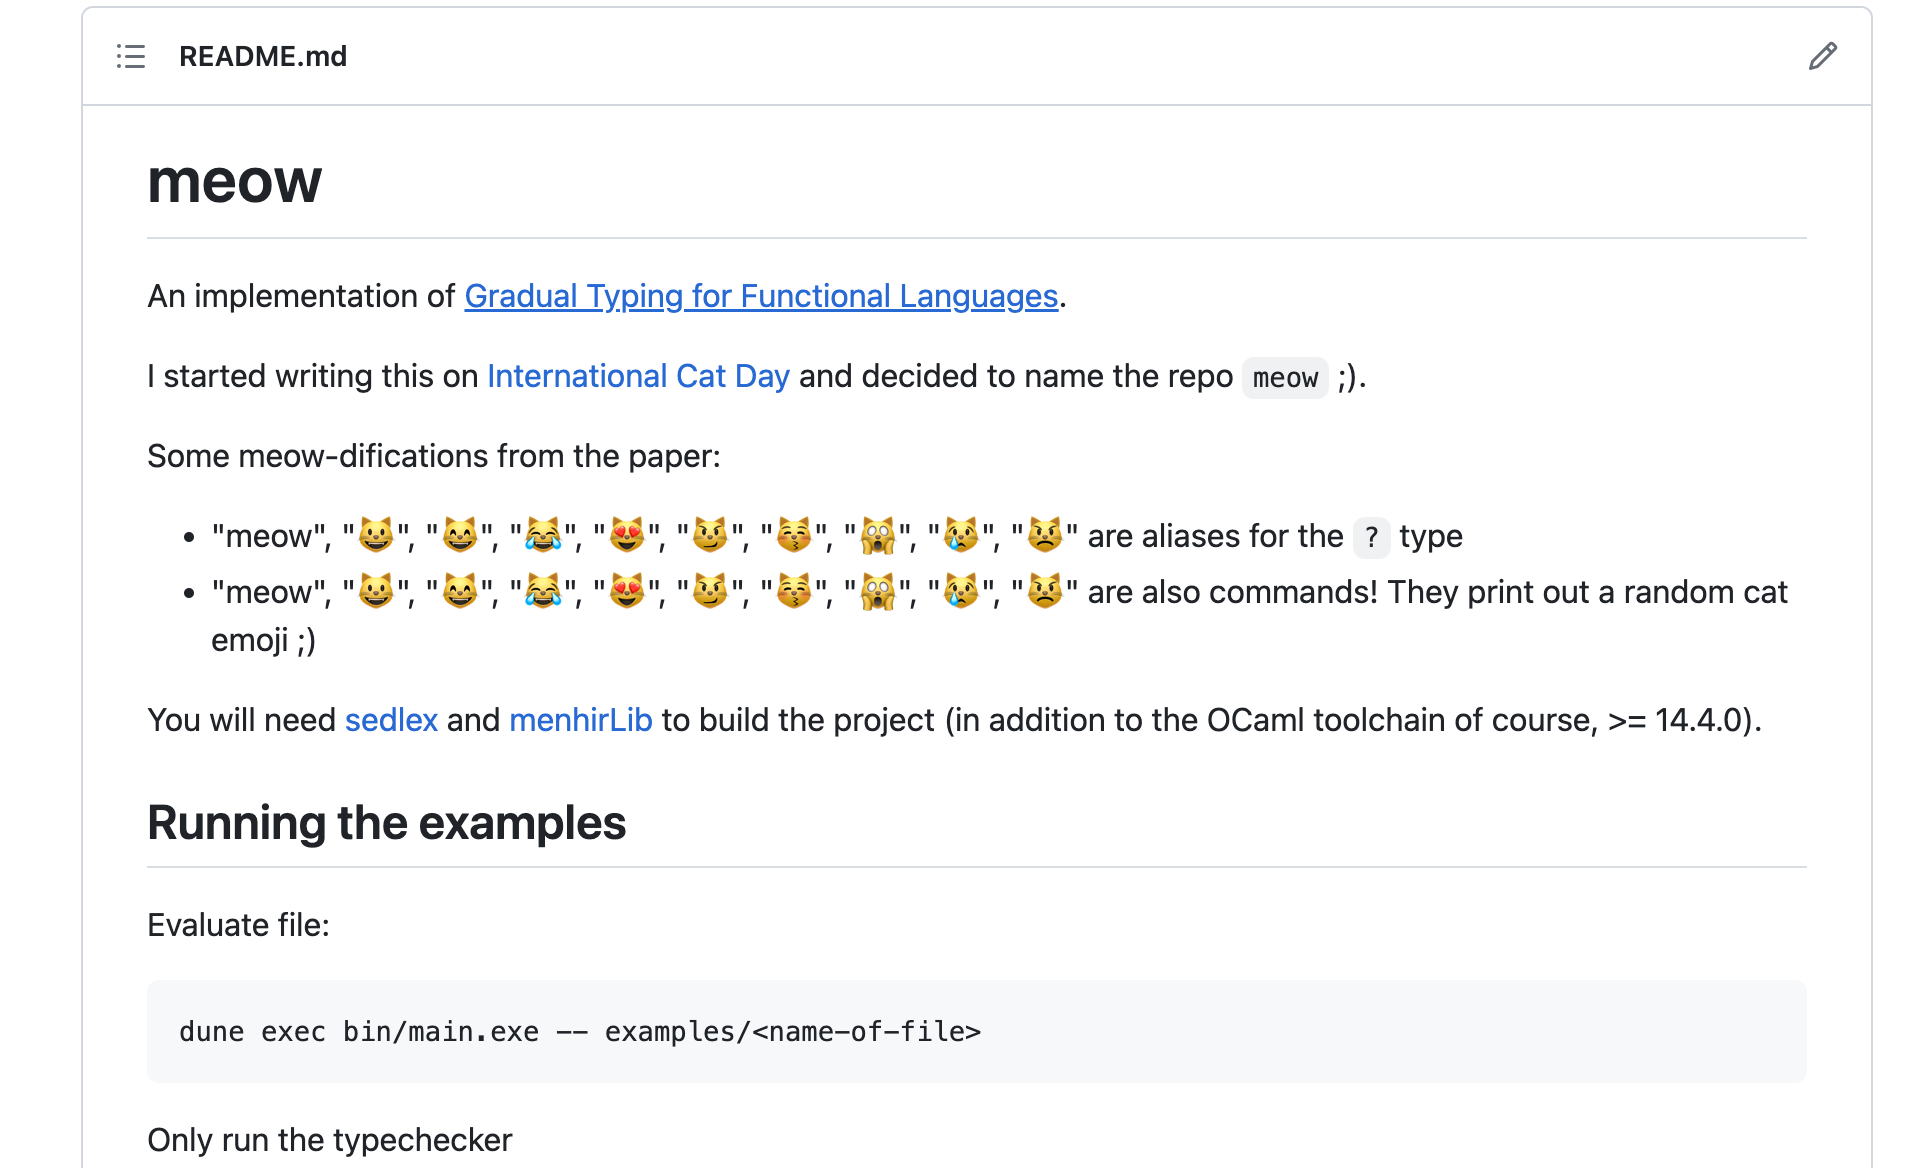
\includegraphics[width=\textwidth]{assets/meow-lang-example}
  \end{figure}
\end{frame}

\begin{frame}{... and learn greek}
  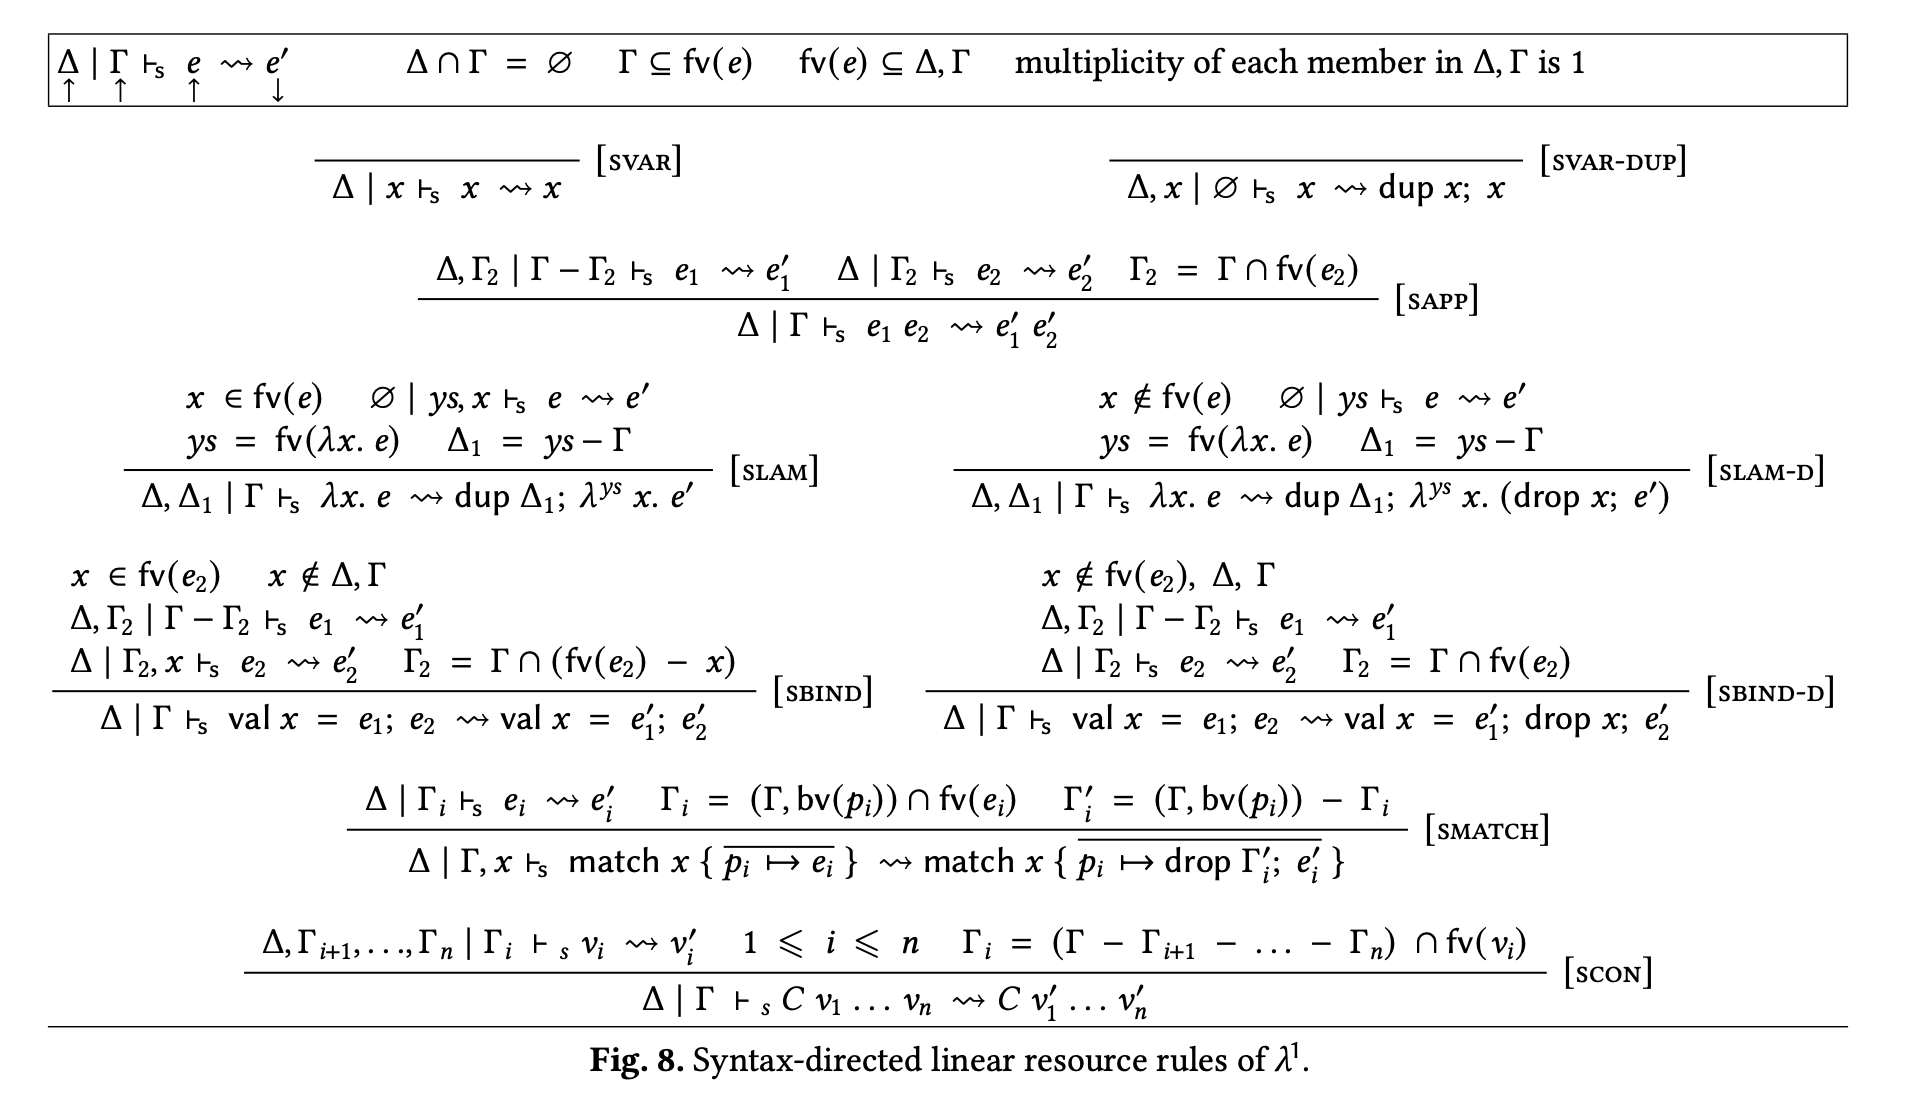
\includegraphics[width=\textwidth]{assets/greek-example}
\end{frame}

\begin{frame}{... and maybe even get to geek about it}
  
\includegraphics[width=\textwidth]{assets/neko-lang-example}
\end{frame}

\begin{frame}{Interested in getting involved?}
  \begin{columns}
    \begin{column}{0.5\textwidth}
      \centering
      Join the discord! \\
      \vspace{1cm}
      \begin{flushleft}
        Contact: \href{mailto://epinto6@gatech.edu}{epinto6@gatech.edu} \\
        Website: \href{https://dtyped.netlify.app}{dtyped.netlify.app}
      \end{flushleft}
    \end{column}
    \begin{column}{0.3\textwidth}
      \centering
      
\includegraphics[width=\textwidth]{assets/join-discord-qr.png}
    \end{column}
  \end{columns}
\end{frame}

\end{document}
